\section{Effect of Neutron Irradiation on Electrical Sensor Properties}
\label{sec:irradiation}

\begin{itemize}
	\item Irradiation worsens electrical properties of silicon sensors.
	\item Effects could be measured, reported in the following.
	\item All based on data with \SI{80}{\min} of annealing at \SI{60}{\celsius}.
	\item Bulk-dominated leakage current per volumne expected to increase proportionally with fluence, investigated in~\ref{subsec:irradiation_alpha}.
	\item Depletion voltage expected to increase, shown in~\ref{subsec:irradiation_Vdep}.
\end{itemize}

\subsection{Current-Related Damage Rate}
\label{subsec:irradiation_alpha}

\begin{itemize}
	\item Leakage currents normalised by volume, scaled to \SI{-20}{\celsius}, cf.~\ref{eq:temp_scaling}
	\item Observe: Proportionality, constant referred to as $\alpha$, cf.~\ref{plot:alpha_Udep,plot:alpha_600}
	\item Report three different alpha values: one around full depletion, one at \SI{600}{\volt} and the third at highest bias voltage of \SI{800}{\volt} (corresponding to end of HGCAL lifetime)
	\item Observe: Independence on sensor production parameters, consistent with previous findings, e.g.~\cite{moll:SiDamages}
	\item All $\alpha$ constants underestimated, w.r.t. literature values
	\item Could possibly hint at overestimate of irradiation fluences at RINSC
\end{itemize}

\begin{figure}
	\captionsetup[subfigure]{aboveskip=-1pt,belowskip=-1pt}
	\begin{subfigure}[b]{0.49\textwidth}
		\centering
		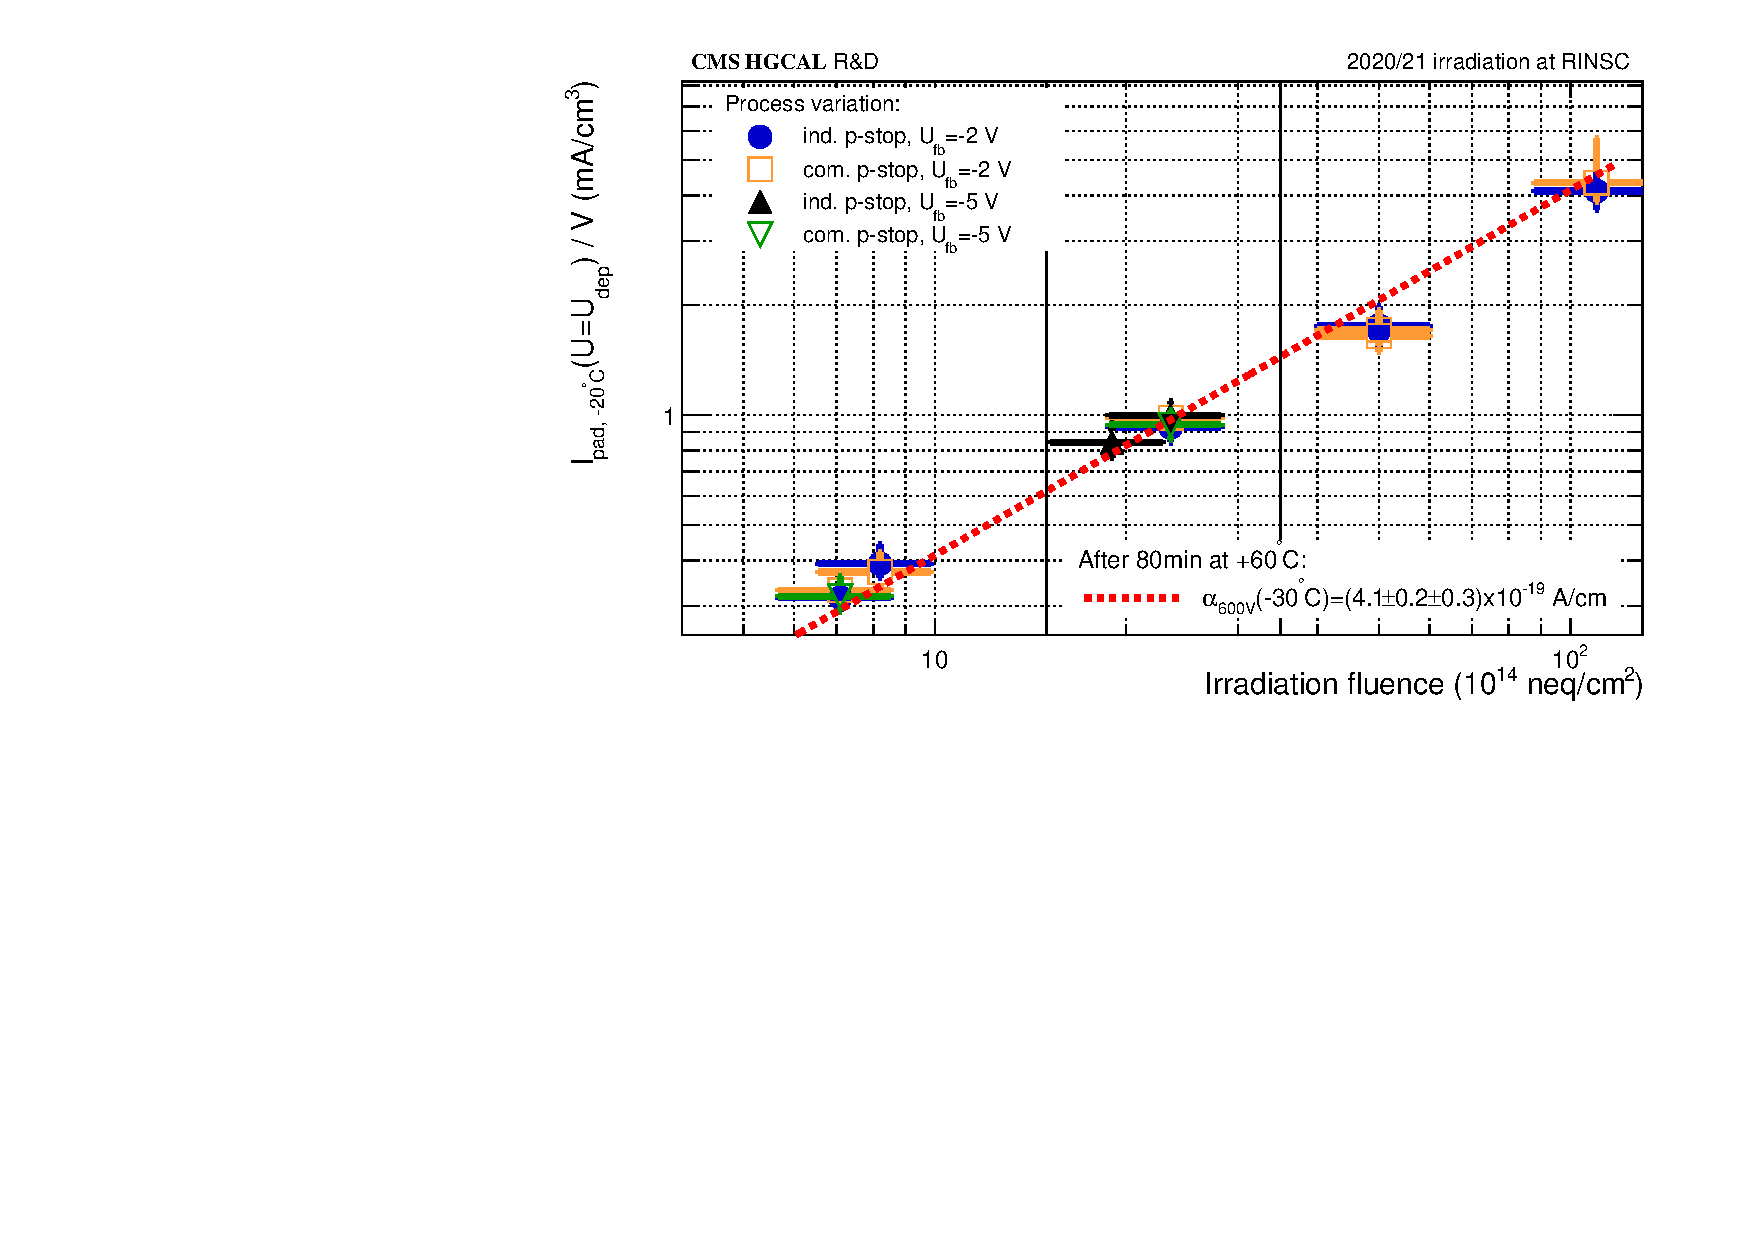
\includegraphics[width=0.99\textwidth]{plots/alpha/alpha_Udep.pdf}
		\subcaption{
			}
			\label{plot:alpha_Udep}
	\end{subfigure}		
	\hfill
	\centering
	\begin{subfigure}[b]{0.49\textwidth}
		\centering
		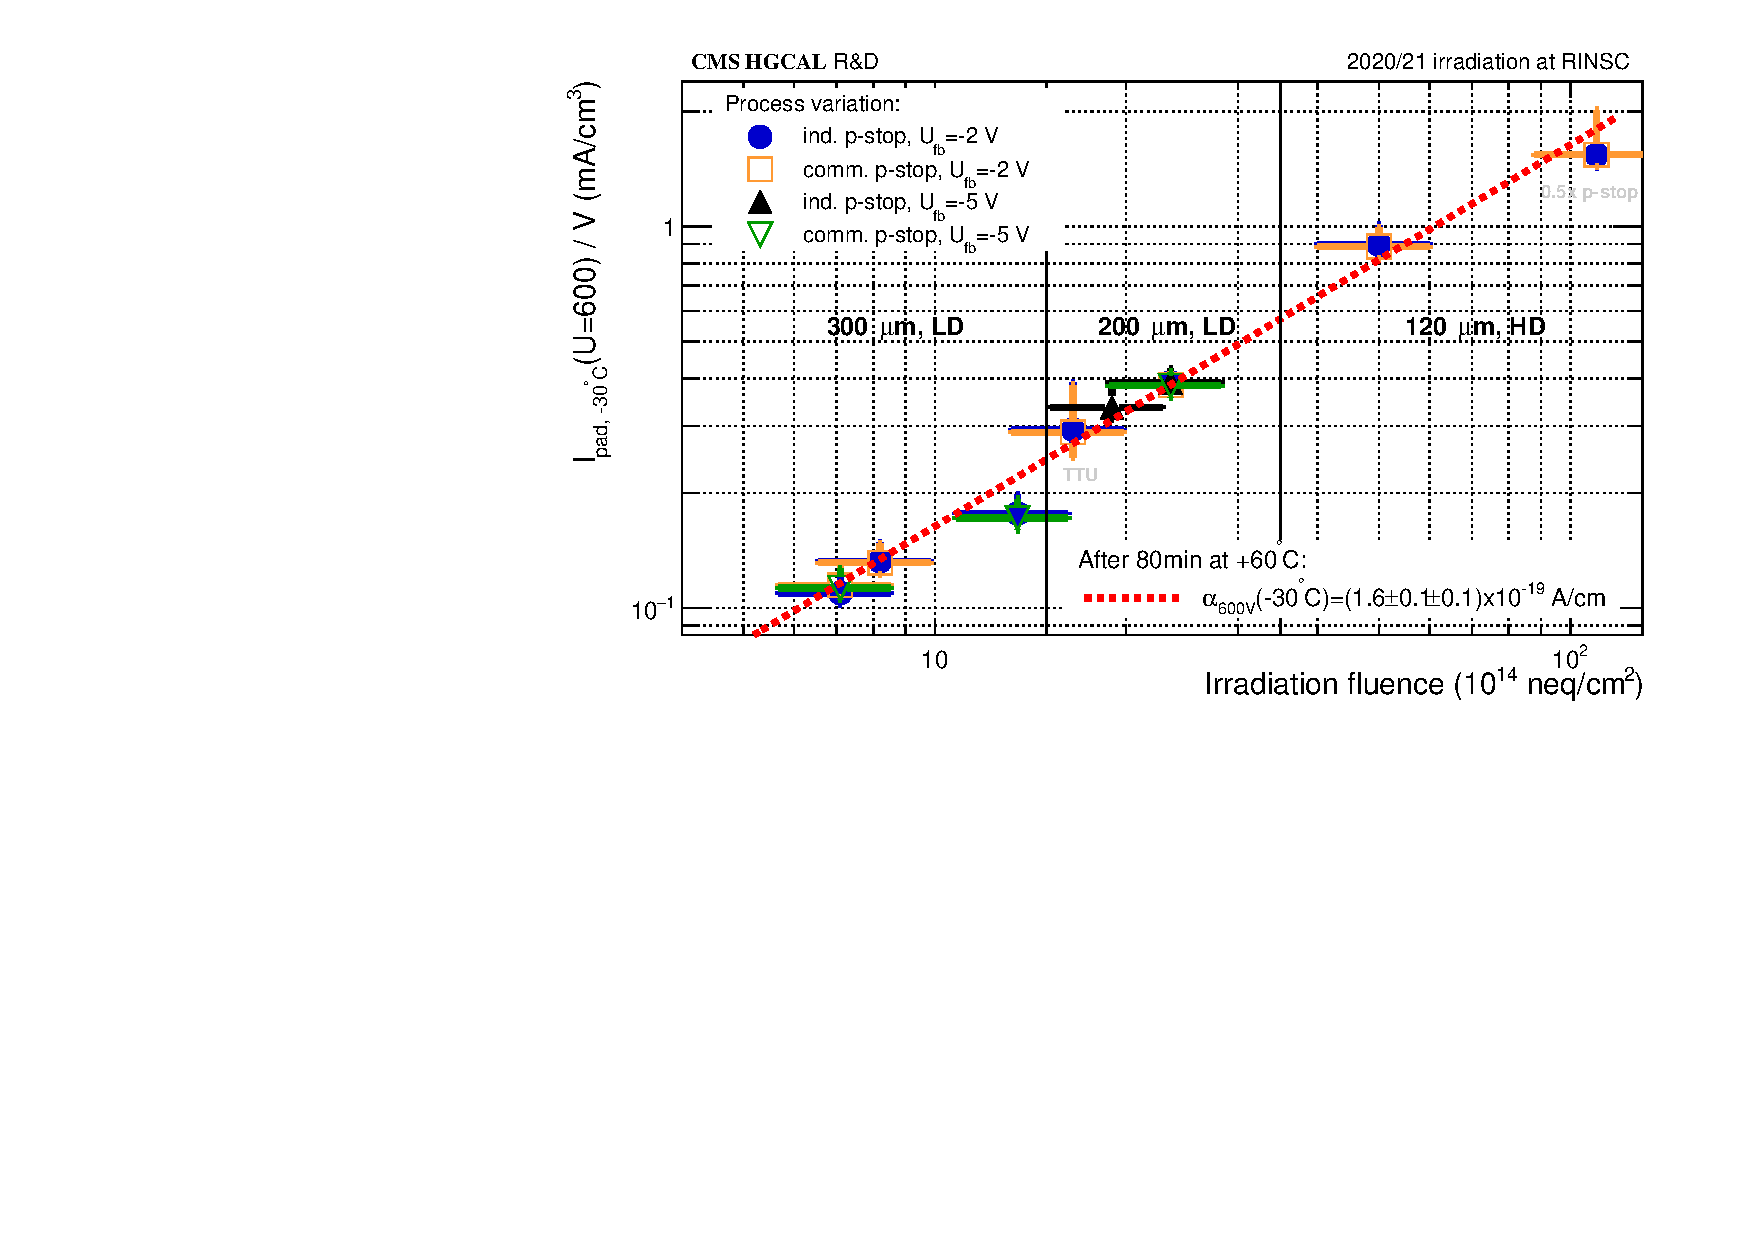
\includegraphics[width=0.99\textwidth]{plots/alpha/alpha_600V.pdf}
		\subcaption{
			}
			\label{plot:alpha_600}
	\end{subfigure}
	\caption{
	    Volume-normalised per-pad leakage current for different fluences (a) at the estimated depletion voltage (using $f_\text{LCR}=\SI{2}{\kilo\hertz}$), (b) at a bias voltage of \SI{600}{\volt}.
		Leakage currents were measured after additional annnealing at \SI{60}{\celsius}, and were scaled to a temperature of \SI{-20}{\celsius}.
        The current-relate damage rate ($\alpha$) is found to be independent of the sensor production parameters investigated in this work.
	}
\end{figure}

\subsection{Depletion Voltage}
\label{subsec:irradiation_Vdep}

\begin{itemize}
	\item Unlike leakage current: Depletion voltage vs. fluence do not agree between different sensors (as expected). Reason: sizable dependence on production parameters, e.g. active thickness
	\item To test impact of fluence on $U_\text{dep}$: Exploit leakage current profile (taken proportional to fluence profile) to demonstrate positive correlation of depletion voltage to fluence.
	\item Use per-pad leakage current at \SI{600}{\volt} as proxy for fluence
	\item In fact: Observe positive correlation, cf.~\ref{plot:Vdep_vs_current_5414,plot:Vdep_hexplot_1002}
	\item Proportionality constant depends on thickness but is consistent between sensors with same thicknesses
\end{itemize}

\begin{figure}
	\captionsetup[subfigure]{aboveskip=-1pt,belowskip=-1pt}
	\centering
	\begin{subfigure}[b]{0.32\textwidth}
		\centering
		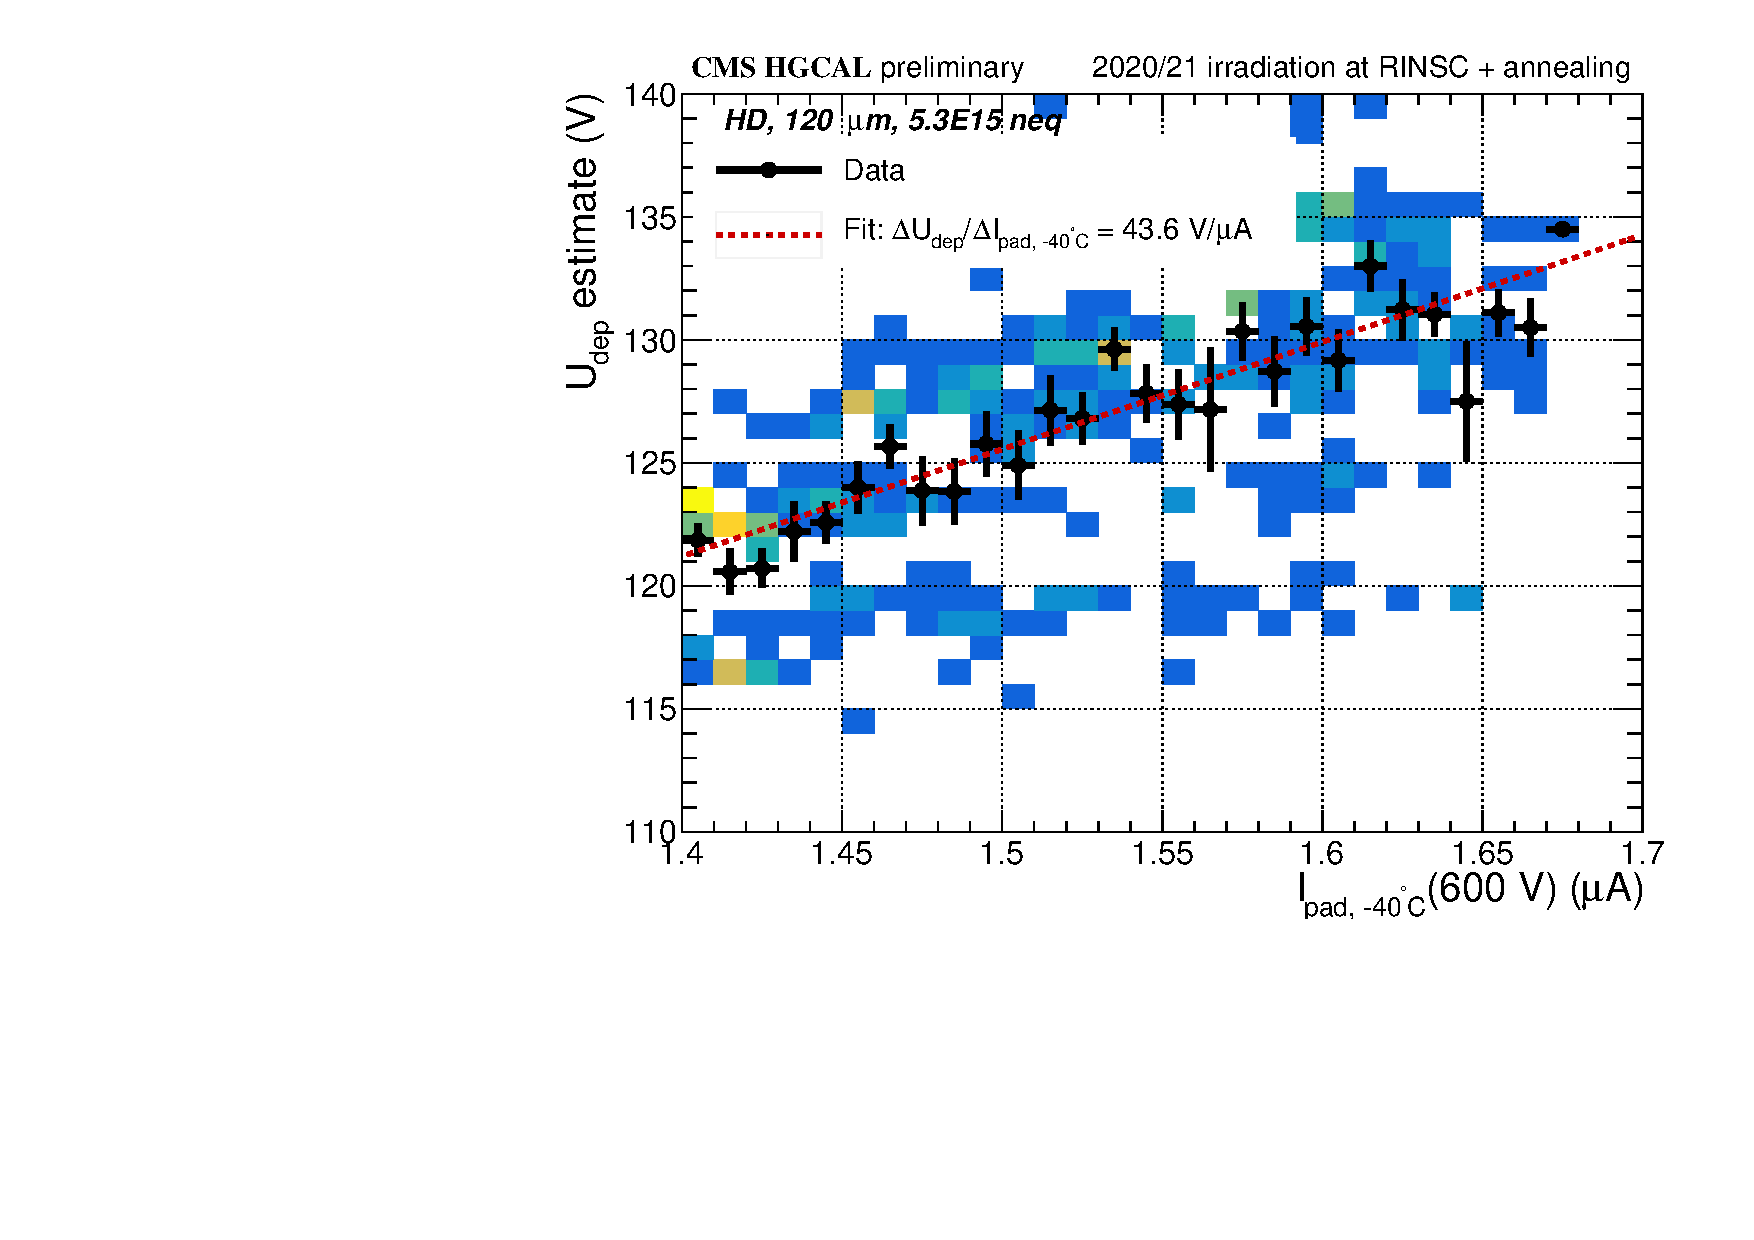
\includegraphics[width=0.999\textwidth]{plots/Vdep_vs_fluence/Vdep_vs_current_3009.pdf}
		\subcaption{
			}
			\label{plot:Vdep_vs_current_3009}
	\end{subfigure}
	\hfill	
	\begin{subfigure}[b]{0.32\textwidth}
		\centering
		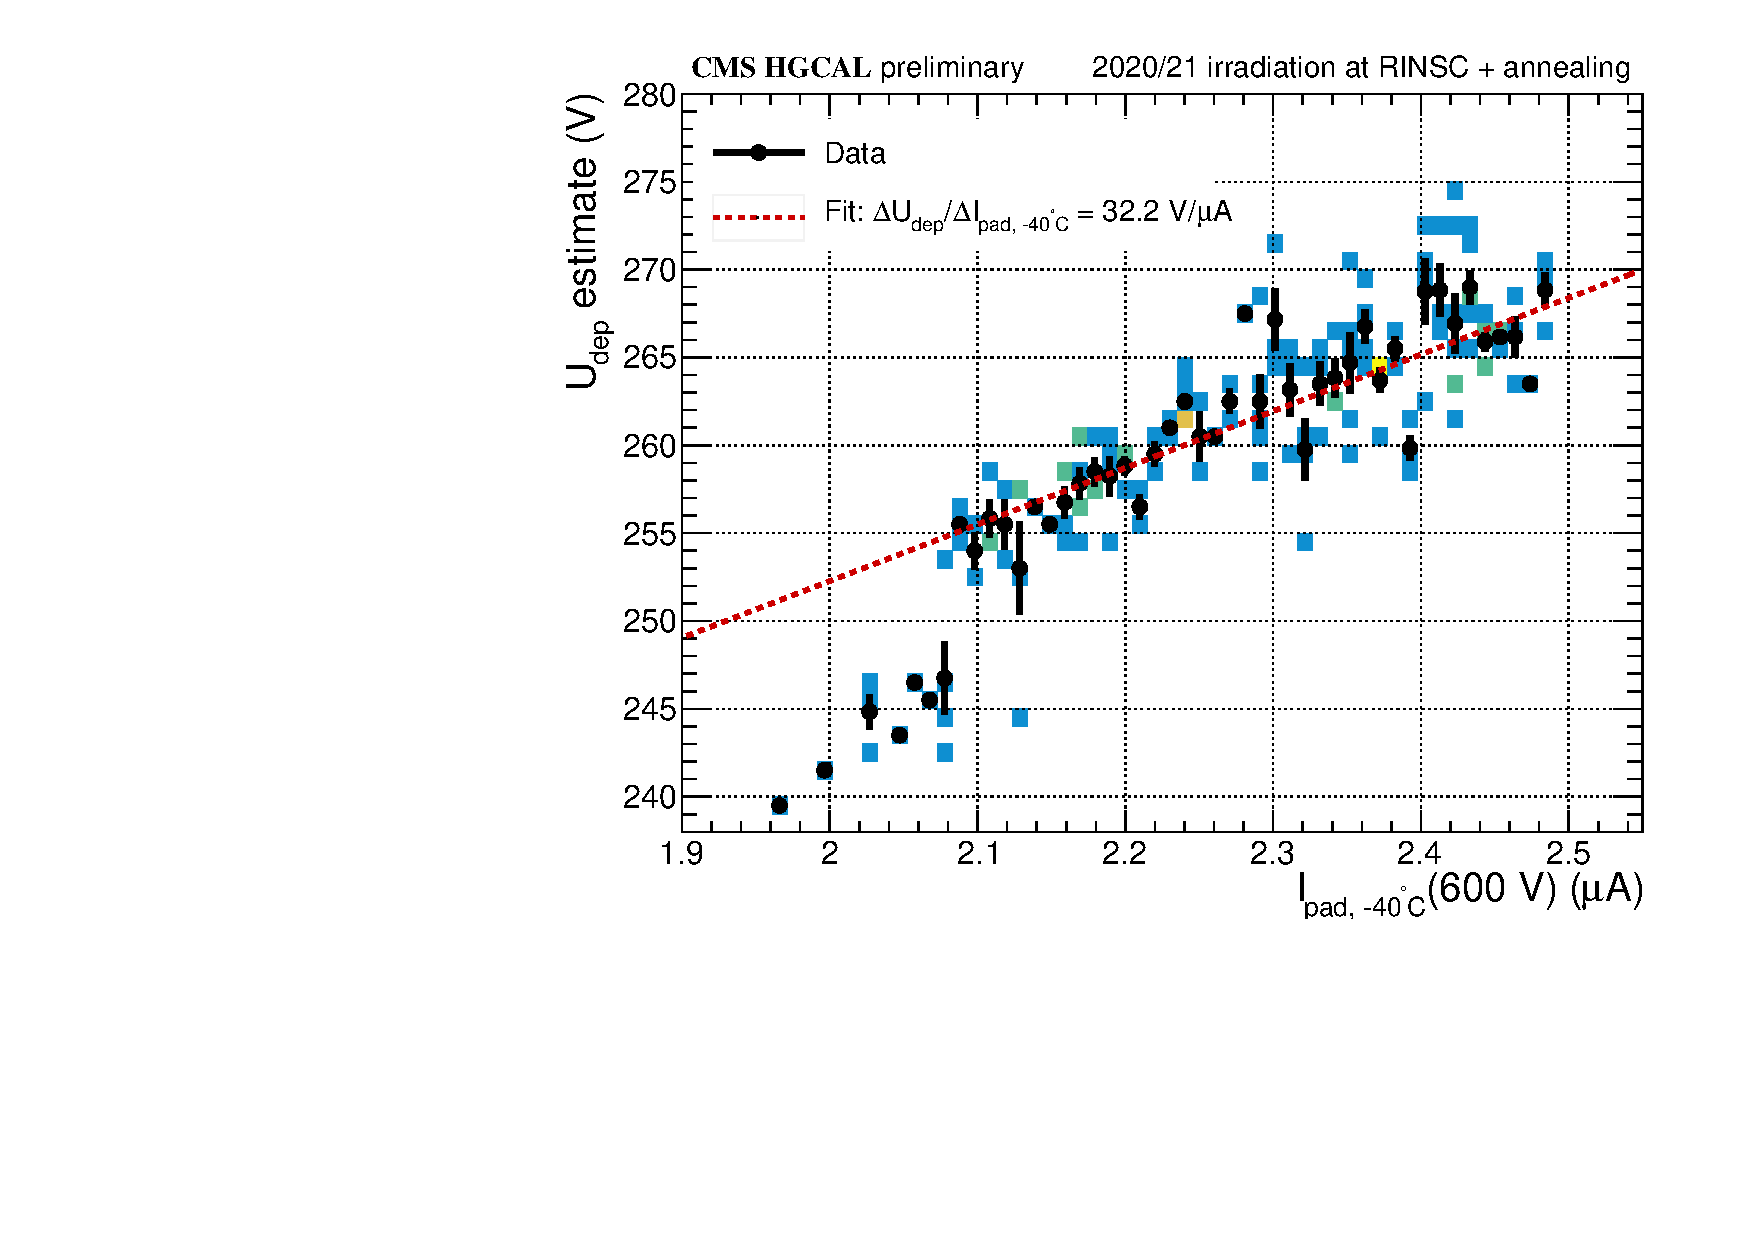
\includegraphics[width=0.999\textwidth]{plots/Vdep_vs_fluence/Vdep_vs_current_5414.pdf}
		\subcaption{
			}
			\label{plot:Vdep_vs_current_5414}
	\end{subfigure}
	\hfill
	\begin{subfigure}[b]{0.32\textwidth}
		\centering
		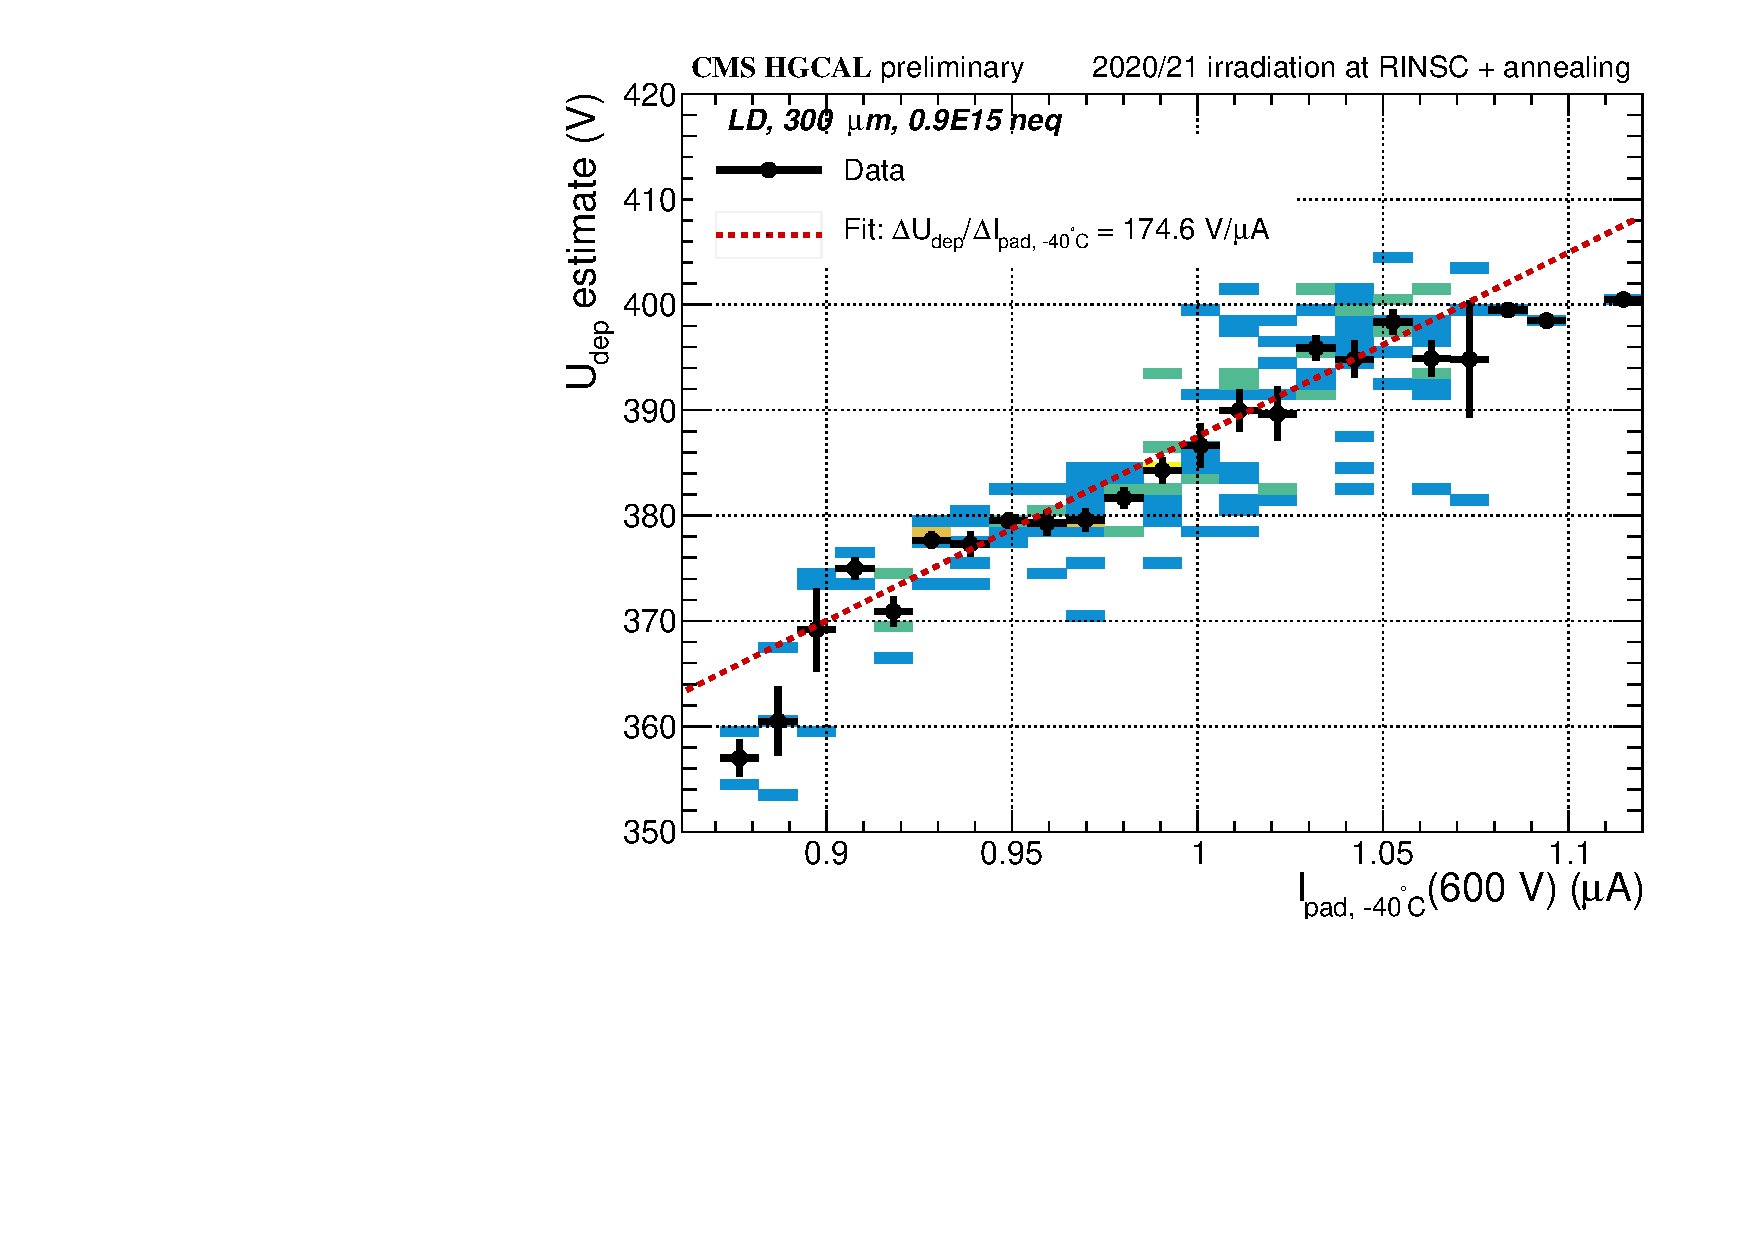
\includegraphics[width=0.999\textwidth]{plots/Vdep_vs_fluence/Vdep_vs_current_1002.pdf}
		\subcaption{
		}
		\label{plot:Vdep_vs_current_1002}
	\end{subfigure}	
	\caption{
		Per-pad depletion voltage estimates vs. per-pad leakage current as proxy for the fluence.
	}
\end{figure}


